\section{Triángulo de Sierpinski}

El proceso para construir el triángulo de Sierpinski consta de reducir el tamaño de un tríangulo equilátero a su cuarta parte de forma que su lado sea la mitad de su lado original, se posicionan tres figuras iguales a esta de manera que formen otro triángulo de lado igual al original. Se repite el mismo proceso para los tres triánguos formados y se vuelve a hacer para todos los nuevos triángulos generados en cada iteración. \cite{Gustavo}

\begin{figure}[H]
    \centering
    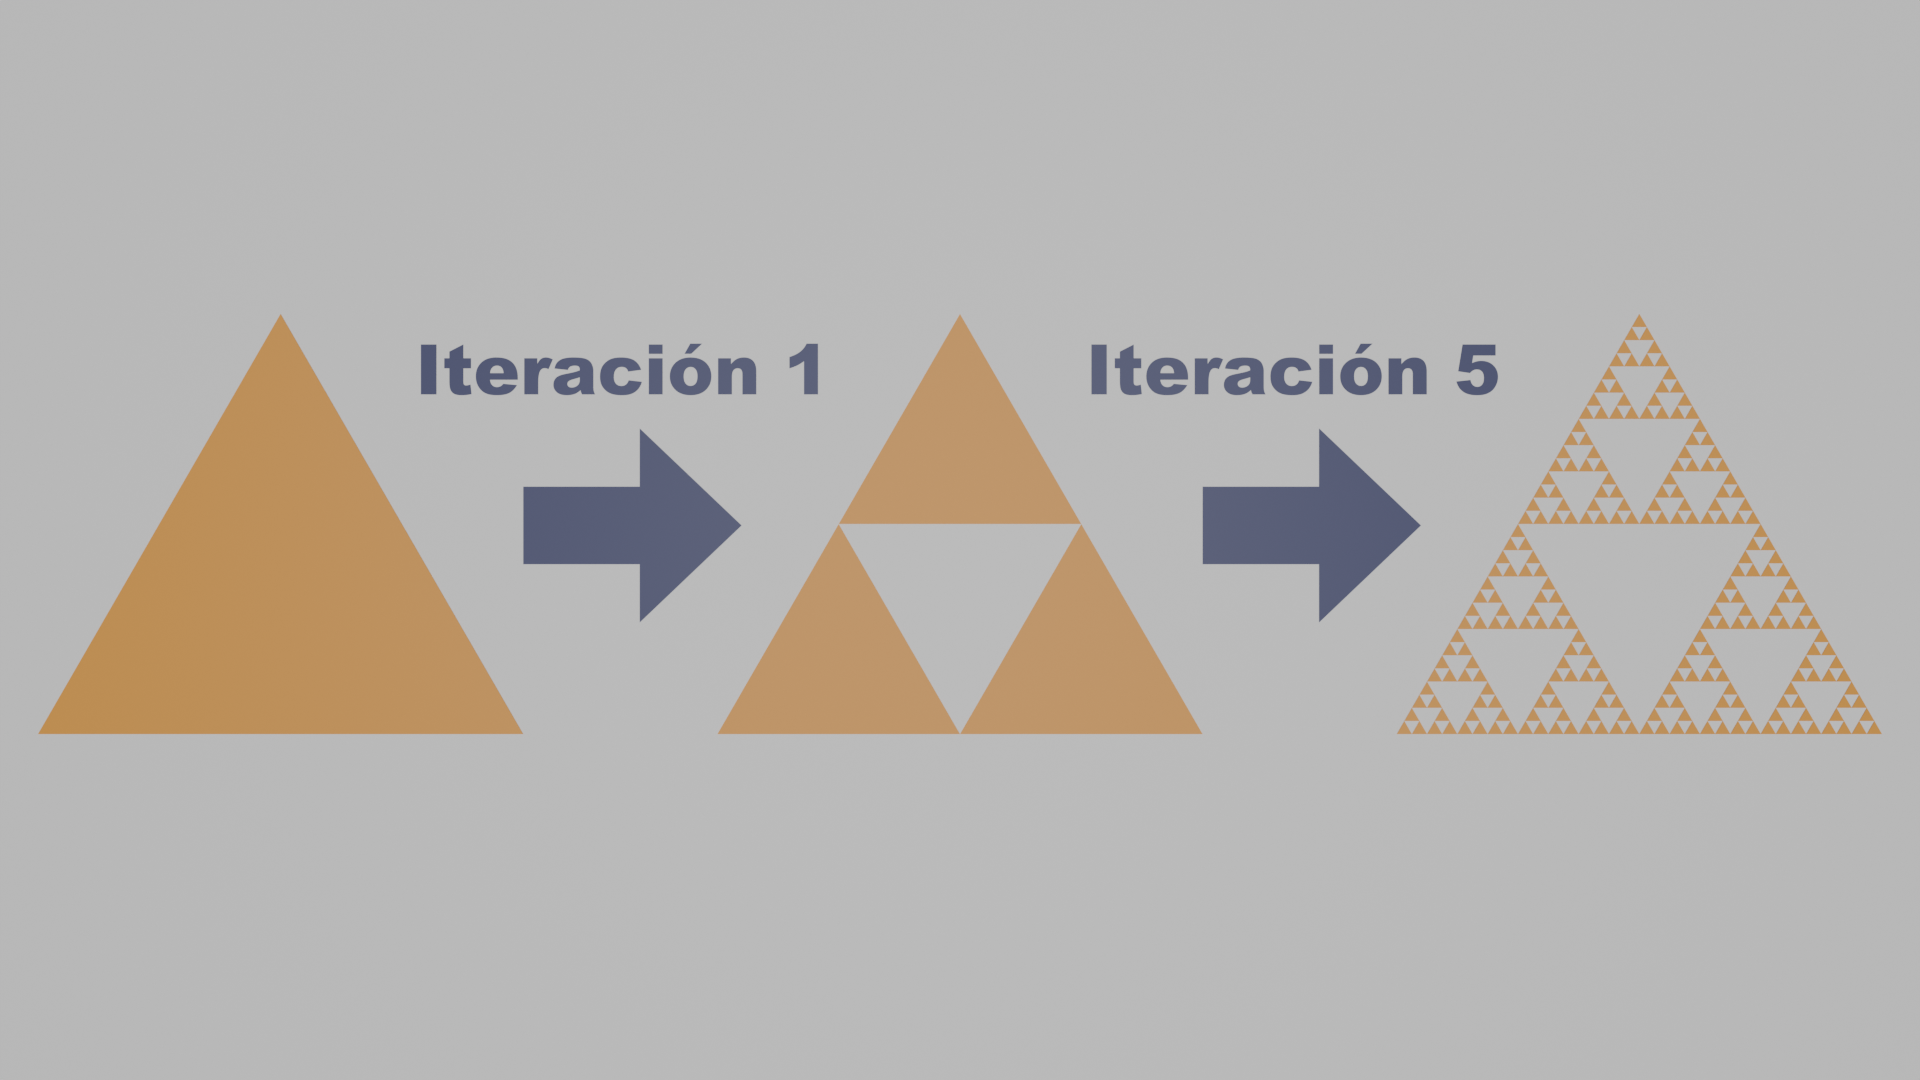
\includegraphics[width=0.5\linewidth]{Figuras/Triangulo.png}
    \caption{Construcción del triángulo de Sierpiński mediante iteraciones sucesivas. Se muestra el triángulo inicial, la primera iteración y la quinta iteración del proceso.}
    \label{fig:triangulo-sierpinski}
\end{figure}